\iffalse
\let\negmedspace\undefined
\let\negthickspace\undefined
\documentclass[journal,12pt,twocolumn]{IEEEtran}
\usepackage{cite}
\usepackage{amsmath,amssymb,amsfonts,amsthm}
\usepackage{algorithmic}
\usepackage{graphicx}
\usepackage{textcomp}
\usepackage{xcolor}
\usepackage{txfonts}
\usepackage{listings}
\usepackage{enumitem}
\usepackage{mathtools}
\usepackage{gensymb}
\usepackage{caption}
\usepackage[breaklinks=true]{hyperref}
\usepackage{tkz-euclide} % loads  TikZ and tkz-base
\usepackage{listings}
\usepackage{gvv}
\newtheorem{theorem}{Theorem}[section]
\newtheorem{problem}{Problem}
\newtheorem{proposition}{Proposition}[section]
\newtheorem{lemma}{Lemma}[section]
\newtheorem{corollary}[theorem]{Corollary}
\newtheorem{example}{Example}[section]
\newtheorem{definition}[problem]{Definition}
%\newtheorem{thm}{Theorem}[section] 
%\newtheorem{defn}[thm]{Definition}
%\newtheorem{algorithm}{Algorithm}[section]
%\newtheorem{cor}{Corollary}
\newcommand{\BEQA}{\begin{eqnarray}}
\newcommand{\EEQA}{\end{eqnarray}}
\newcommand{\define}{\stackrel{\triangle}{=}}
\theoremstyle{remark}
\newtheorem{rem}{Remark}

%\bibliographystyle{ieeetr}
\begin{document}
%

\bibliographystyle{IEEEtran}


\vspace{3cm}

\title{
%  \logo{
GATE AE-54(2023)

\large{EE:1205 \brak{Signals  Systems}}

Indian Institute of Technology, Hyderabad
%  }
}
\author{Md Ayaan Ashraf

EE23BTECH11041
}  
\maketitle
\newpage
\bigskip
\renewcommand{\thefigure}{\arabic{figure}}
\renewcommand{\thetable}{\arabic{table}}
%\renewcommand{\theequation}{\theenumi}
\section*{\textit{\textbf{Question}}}
Consider the differential equation
\begin{align}
x^2\frac{d^2y}{dx^2} + 4x\frac{dy}{dx} + 2y = 0 \quad \text{for } x\geq 1 \nonumber
\end{align}
with initial conditions $y=0$ and $\frac{dy}{dx} = 1$ at
$x = 1$. The value of $y$ at $x = 2$ is ?

\hfill {(GATE AE 2023)}
\solution
\fi
\noindent Given : 
\begin{align}
x^2\frac{d^2y}{dx^2} + 4x\frac{dy}{dx} + 2y = 0 \quad \text{for } x\geq 1 \label{eq:given equation}
\end{align}
Using Euler Substitution : 
\begin{align}
x= & e^t \label{eq:x}\\
\frac{dy}{dx}= & e^{-t}\frac{dy}{dt}\label{eq:dy/dx}\\
\frac{d^2y}{dx^2} = & e^{-2t}\frac{d^2y}{dt^2} - e^{-2t}\frac{dy}{dt}\label{eq:d^2y/dx^2}
\end{align}
Substituting equations \eqref{eq:x},\eqref{eq:dy/dx},\eqref{eq:d^2y/dx^2} in equation \eqref{eq:given equation}:
\begin{align}
\frac{d^2y}{dt^2} + 3\frac{dy}{dt} + 2y = 0
\end{align}
Taking Laplace on Both Sides:
\begin{align}
s^2 Y(s) - sy(1)-y'(1) + 3{sY(s) - y(1)} + 2Y(s)= 0\label{eq:laplace}
\end{align}
We know that:
\begin{align}
y(1)=0\label{eq:given 1}\\
y'(1)=1\label{eq:given 2}
\end{align}
Substituting equations \eqref{eq:given 1},\eqref{eq:given 2} in \eqref{eq:laplace}
\begin{align}
s^2Y(s)& + 3sY(s) +2Y(s)= 1\\
\implies Y(s)=&\frac{1}{s^2 + 3s + 2 }\\
\implies Y(s)=&\frac{1}{s+1} - \frac{1}{s+2}
\end{align}
Taking Inverse Laplace:
\begin{align}
y(t) = (e^{-t} - e^{-2t})u(t)
\end{align}
Substituting $x=e^t$:
\begin{align}
y(x)=& e^{-\ln{x}} - e^{-2\ln{x}},\quad x\geq 1 \\
y(x)=& \frac{1}{x} - \frac{1}{x^2},\quad x\geq 1 
\end{align}
\begin{align}
    \therefore y(2) = 0.25
\end{align}
\begin{figure}[ht]
    \centering
    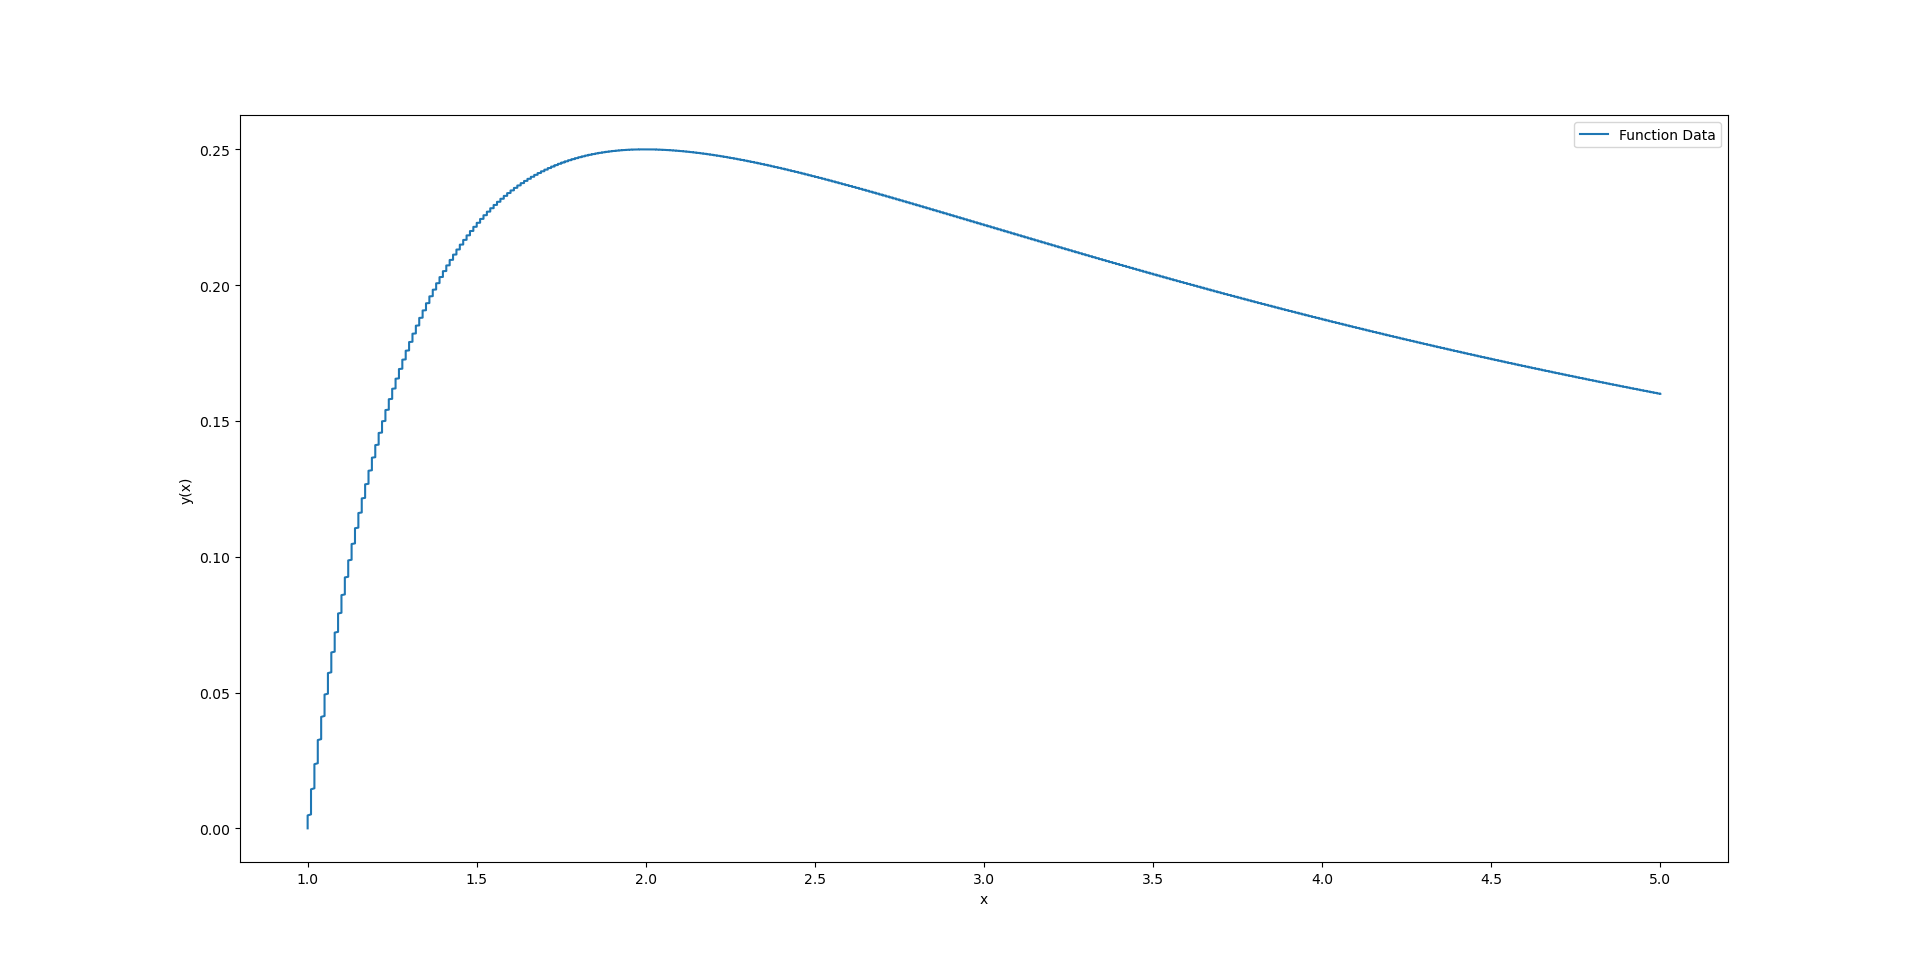
\includegraphics[width=\columnwidth]{2023/AE/54/figs/fig.png}
    \caption{Plot of $y(x)$ $vs$ $x$}
    \label{fig: GATE AE-54(2023)}
\end{figure}
